\documentclass[main.tex]{subfiles}
%\usepackage{tikz}
%\usetikzlibrary{positioning,calc}
%\usepackage{pgfplots}

\begin{document}
\subsubsection{Photo Policy Acknowledgement on Moodle}

On Moodle, under the section for this lab, carefully review and respond to the Photo Policy Acknowledgement. \textbf{You will not be able to get credit for the other activities OR the lab project until you do!}

\subsubsection{Angular sizes}
We will use a uniform grid to get a sense of how to consistently compare the angular sizes we see.
\begin{enumerate}
\item Stand with your eye/camera located 12 ft from the screen. Look at the floor plan to determine where you should stand. At this distance, the squares on the grid are \SI{1}{\degree} wide on each side.
\item Try out things you can use to estimate different angles, e.g., your outstretched hand, your thumb, a credit card, a coin, a key, or even a cell phone that you always have with you. Write down what you use and sketch how they appear on the grid.

Be consistent! E.g., if you are using 4 fingers at arm's length, always hold them out at full arm's length.

\end{enumerate}

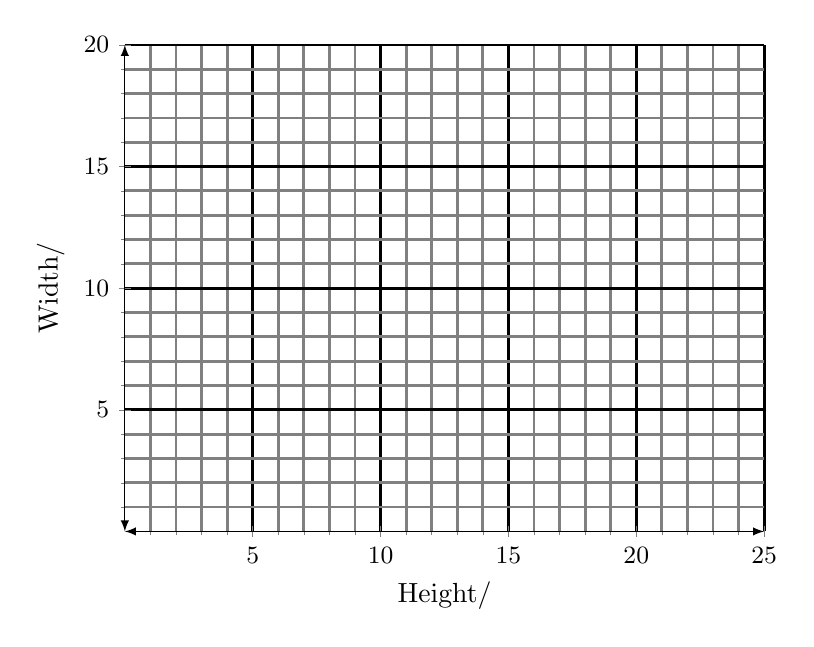
\begin{tikzpicture}
\begin{axis}[
	width=0.8\textwidth,
    height=0.64\textwidth,
    xmin=0,xmax=25,xtick={0,5,10,15,20,25},minor xtick={1,2,3,4,6,7,8,9,11,12,13,14,16,17,18,19,21,22,23,24},
    ymin=0,ymax=20,ytick={0,5,10,15,20},minor ytick={1,2,3,4,6,7,8,9,11,12,13,14,16,17,18,19},
    grid=both,
    grid style={line width=1pt, draw=gray!100},
    major grid style={line width=1pt, draw=black!100},
    axis lines=center,
    minor tick num=1,
    %enlargelimits={abs=0.5},
    axis line style={latex-latex},
    ticklabel style={font=\small},
    xlabel near ticks,
    ylabel near ticks,
    xlabel={Height/\si{\degree}},
    ylabel={Width/\si{\degree}}
]
\end{axis}
\end{tikzpicture}

\begin{center}
\begin{tabular}{|l|p{3cm}|p{3cm}|p{3cm}|p{3cm}|}\hline
Size & \SI{1}{\degree} & \SI{5}{\degree} & \SI{10}{\degree} & \SI{20}{\degree}\\\hline
Object&&&&\\
&&&&\\\hline
\end{tabular}
\end{center}

\subsubsection{Calibrating your camera (angular field of view)}
At a set zoom level (as well as picture size i.e. height/width ratio), your camera will always cover the same angular dimensions. This is also often known as a \textbf{field of view}. Let's find out what they are by calibrating your camera.

\begin{enumerate}
\item Hold your camera at the same position as before, i.e. 12 ft from the screen. Make sure your \textbf{camera} is located at the 12 ft mark.
\item Zoom in as far as you can on your camera.
\item Take a photo of the grid. Try to align it with the screen.
\item Count the number of squares on each side of your picture. This will give you the angular size of each side.
\item Record all your findings and settings below.
\end{enumerate}

\begin{center}
\begin{tabular}{|p{2.5cm}|p{3cm}|p{4cm}|p{4cm}|}\hline
Zoom level & Other settings & Angular size: Height & Angular size: Width\\\hline
&&&\\
&&&\\\hline
\end{tabular}
\end{center}

Now let's use what we've learnt to do some astronomy! First, we'll use the visual estimates from the second section.

\begin{enumerate}
\item Look at the Stellarium view projected on the screens. It simulates a real-life view of the night sky at the same scale as the grid before. 
\item Use similar things to those in Part 1 (fingers, coin, etc.) to estimate angular sizes and answer the questions below. \textbf{Remember to be consistent! Hold your arm out at full length!}
\begin{enumerate}
\item How many degrees is Aldebaran from the Pleiades cluster of stars?\\

\rule{14cm}{.2mm}
\item Which of your angular measures (such as hand, thumb, pencil) is most similar in angular width as the Pleiades?\\

\rule{14cm}{.2mm}
\item How many times wider is your outstretched finger than the Moon?\\

\rule{14cm}{.2mm}
\end{enumerate}
\item Take a photo of the projected Moon like you did for the grid:
	\begin{itemize}
	\item Fully zoomed in
	\item Held at 12 ft from screen
	\end{itemize}
\item Compare it with your calibration picture and calibrated values. How big is the Moon?\\

\rule{15cm}{.2mm}
\end{enumerate}

\subsubsection{Taking a zoom back}
Now let's calibrate your camera fully zoomed out. 
\begin{enumerate}
\item Zoom out on your camera to 1x. \textbf{If your camera has 0.5x zoom or similar, do not use it.}
\item Take a photo of the grid from 12 ft. You'll see that the screen appears much smaller. Compared to before, when your camera was zoomed in, approximately how many times wider and taller is your camera field of view now? How does this compare to your previously recorded zoom level?\\

\rule{15cm}{.2mm}
\item Move your camera approximately 3 ft from the screen using a yardstick.  
\item Take a photo of the \text{new} grid, which has lines every \SI{5}{\degree}.
\item Count the number of squares on each side of your picture \textbf{and multiply that number by 5}. This will give you the angular size of each side.
\item Record all your findings and settings below.
\end{enumerate}

\begin{center}
\begin{tabular}{|p{2.5cm}|p{3cm}|p{4cm}|p{4cm}|}\hline
Zoom level & Other settings & Angular size: Height & Angular size: Width\\\hline
&&&\\
&&&\\\hline
\end{tabular}
\end{center}

As you end up standing $4\times$ closer to the screen, the projected grid has cover an area that is $4\times$ taller AND $4\times$ wider in order to be consistent. In general, when you get $x$ times closer to an object, its angular size will get $x$ times bigger.

Now, we'll look at a simulation of a sunset view, similar to the pictures you'll be asked to take for the sunset project.

\begin{enumerate}
\item Look at the Stellarium view projected on the screens. It simulates a real-life view shortly before sunset.
\item With your camera 3 ft from the screen, take a photo of the screen.
\item Compare it with your calibration picture and calibrated values to find the following, keeping in mind that the azimuth of due west is \SI{270}{\degree}.
\begin{center}
\begin{tabular}{|p{3cm}|p{4cm}|}\hline
Azimuth of Sun & \\
&\\\hline
Altitude of Sun & \\
&\\\hline
\end{tabular}
\end{center}
\end{enumerate}

\subsubsection{Moodle Lab Quiz}
Go to the section for this lab on the Moodle page and complete the End-of-Lab Quiz and upload your calibration pictures on Moodle by the end of the week. Also, remember to fill out the Photo Policy Acknowledgement.

If you switch to a new camera or change your settings, let your TAs know. There will be opportunities to re-calibrate your camera with the grids in future labs.

\end{document}